% !Mode:: "TeX:UTF-8"

%Composed by Y.B. TANG (ybtang21c@gmail.com), spring-2011
%tex distribution: Texlive / MikTex 2010
%recommended editer: Eclipse + Texlipse
%usage: compile with XeLatex

%option: red, brown, blue
\documentclass[a4paper]{article}

\usepackage{amsmath,amsfonts,amssymb,amsthm,bm}
% \usepackage{txfonts} %another style of math fonts
\usepackage{color,graphics}
\usepackage{ulem} %erase line

% ==============std fontspec settings==============
\usepackage[no-math,cm-default]{fontspec}
\newfontfamily\zhfont[BoldFont=Adobe Heiti Std]{Adobe Kaiti Std}

% ==============spacing of CH in Xetex==============
\usepackage{zhspacing}
\zhspacing

%==============layout setting==============
\setlength{\parindent}{0pt}

%=============test========================

\usepackage[left={3cm},right={4cm},marginparwidth={3cm},marginparsep={1em},vmargin={2cm},]{geometry}%
% \usepackage{amsmath,amsthm,amscd,amssymb,graphicx,comment,enumerate,picins,ifthen,multicol,fancyvrb,listings,color,verbatim}
\usepackage{fancyhdr}

\pagestyle{fancy} \columnsep=10mm

% \fancyhead[RE]{\leftmark} % 在偶数页的右侧显示章名
\fancyhead[LO]{\rightmark} % 在奇数页的左侧显示小节名
% \fancyhead[LE,RO]{~\thepage~} % 在偶数页的左侧,奇数页的右侧显示页码
% \fancyfoot[RO,RE]{\it 国防科学技术大学-理学院}
\renewcommand{\baselinestretch}{1.5}
\renewcommand{\headrulewidth}{0pt}
% \usepackage[CJKbookmarks=true,bookmarksnumbered,bookmarksopen,colorlinks,linkcolor=blue,anchorcolor=blue,citecolor=green,dvipdfm]{hyperref}
% \excludecomment{student}
% \includecomment{teacher}

%===============macros====================
\newcommand{\bb}{\bf\color{blue}}
\newcommand{\ba}[1]{\alert{\bf #1}}
\newcommand*{\e}{\ensuremath{\varepsilon}}
\renewcommand{\b}{\color{blue}}
\newcommand*{\p}{\ensuremath{\partial}}
\newcommand{\limn}{\ensuremath{\lim\limits_{n\to\infty}}}
\newcommand{\sumn}{\ensuremath{\sum\limits_{n=1}^{\infty}}}
\newcommand*{\df}[2]{\displaystyle\frac{\,{#1}\,}{\,{#2}\,}}
\newcommand*{\limx}[1]{\ensuremath{\lim\limits_{x\to{#1}}}}
\newcommand*{\limdx}{\ensuremath{\lim\limits_{\Delta x\to 0}}}
\newcommand*{\dx}{\Delta x}
\newcommand{\dint}{\ensuremath{\displaystyle\int}}
\renewcommand{\d}{\mathrm{d}}


%===============document begins here==============

\begin{document}

%0.3.7:系赛最终版
%0.3.9:院赛

%    \begin{frame}
	\titlepage
\end{frame}

\begin{frame}{平面曲线的曲率}
	\linespread{1.5}
	\begin{columns}
		\column{.5\textwidth}
			\vspace{-2cm}
			\begin{itemize}
		      \item {\bf 平面曲线的曲率概念}
		      \item {\bf 曲率的计算公式}
		      \item {\bf 曲率圆与曲率的应用}
		    \end{itemize}
		\column{.5\textwidth}
			\vspace{2cm}
			\resizebox{!}{5cm}{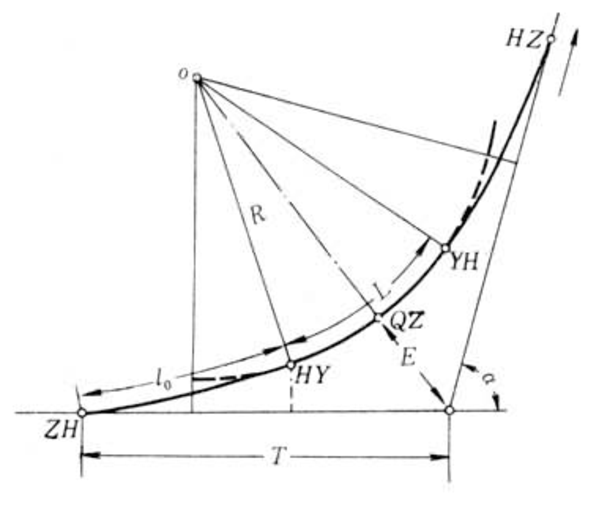
\includegraphics{./images/tcs.pdf}}
	\end{columns}
\end{frame}

\begin{frame}{铁路的设计}
	\linespread{1.2}
	\begin{center}
		\resizebox{!}{7cm}{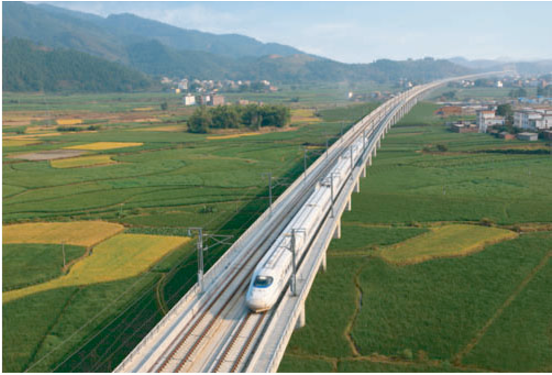
\includegraphics{./images/rw1.pdf}}
	\end{center}
\end{frame}

\begin{frame}{复习与回顾}
	\linespread{1.5}
	\ba{如何刻画一条平面曲线的几何特征?}
	
	\begin{enumerate}
	  \item {\bf 切线斜率:}一阶导数
	  \item {\bf 凹凸性:}二阶导数
	  \item {\bf 长度:}弧微分\pause
	  \item {\bf 弯曲程度:}{\b 曲率}
	\end{enumerate}
\end{frame}

\section{曲率}

\subsection{曲率的概念}

\begin{frame}{曲率}
	\linespread{1.2}
	\centerline{\ba{如何刻画曲线的弯曲程度?}}
	\pause
	\begin{columns}
		\column{.5\textwidth}
			\begin{center}
				\vspace{-1em}
				{\resizebox{!}{5.5cm}{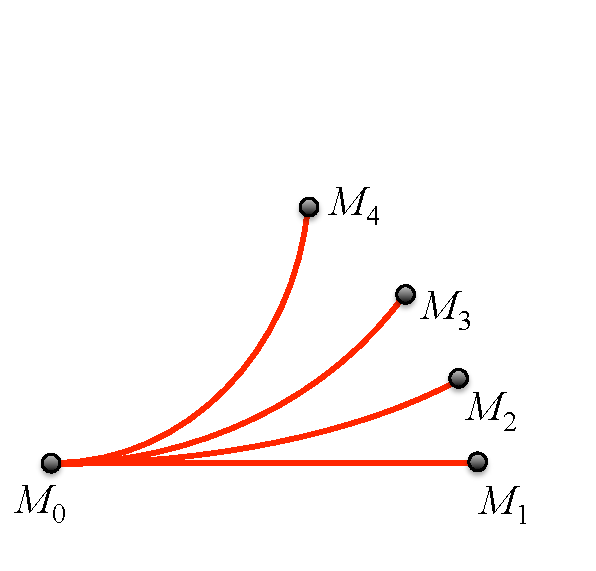
\includegraphics{./images/curves/c106.pdf}}}

				\vspace{-1em}\invisible<1->{{\b 长度相同的曲线,切线

				转角越大弯曲程度越大}}
			\end{center}
		\column{.5\textwidth}
	\end{columns}
\end{frame}

\begin{frame}{曲率}
	\linespread{1.2}
	\centerline{\ba{如何刻画曲线的弯曲程度?}}

	\begin{columns}
		\column{.5\textwidth}
			\begin{center}
				\vspace{-1em}
				{\resizebox{!}{5.5cm}{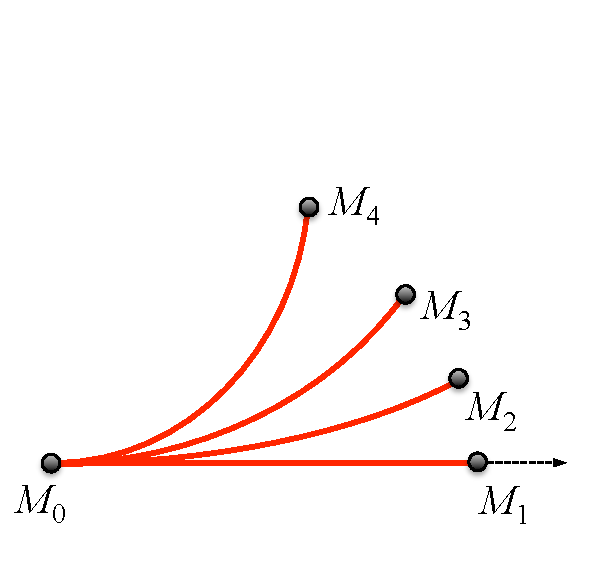
\includegraphics{./images/curves/c105.pdf}}}

				\vspace{-1em}\invisible<1->{{\b 长度相同的曲线,切线

				转角越大弯曲程度越大}}
			\end{center}
		\column{.5\textwidth}
	\end{columns}
\end{frame}

\begin{frame}{曲率}
	\linespread{1.2}
	\centerline{\ba{如何刻画曲线的弯曲程度?}}

	\begin{columns}
		\column{.5\textwidth}
			\begin{center}
				\vspace{-1em}
				{\resizebox{!}{5.5cm}{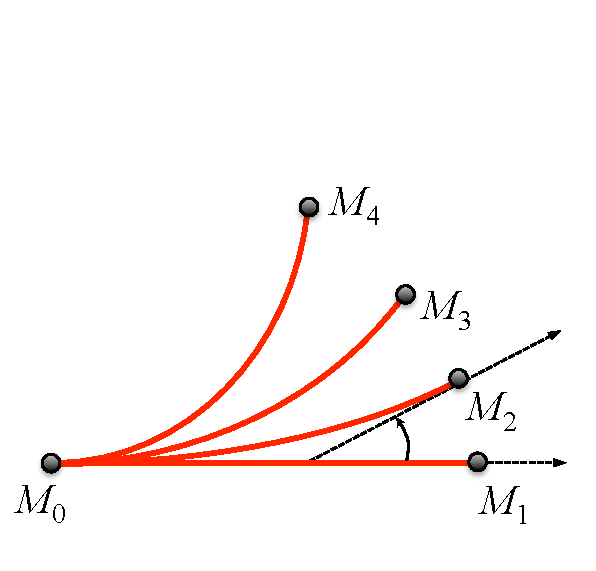
\includegraphics{./images/curves/c104.pdf}}}

				\vspace{-1em}\invisible<1->{{\b 长度相同的曲线,切线

				转角越大弯曲程度越大}}
			\end{center}
		\column{.5\textwidth}
	\end{columns}
\end{frame}

\begin{frame}{曲率}
	\linespread{1.2}
	\centerline{\ba{如何刻画曲线的弯曲程度?}}

	\begin{columns}
		\column{.5\textwidth}
			\begin{center}
				\vspace{-1em}
				{\resizebox{!}{5.5cm}{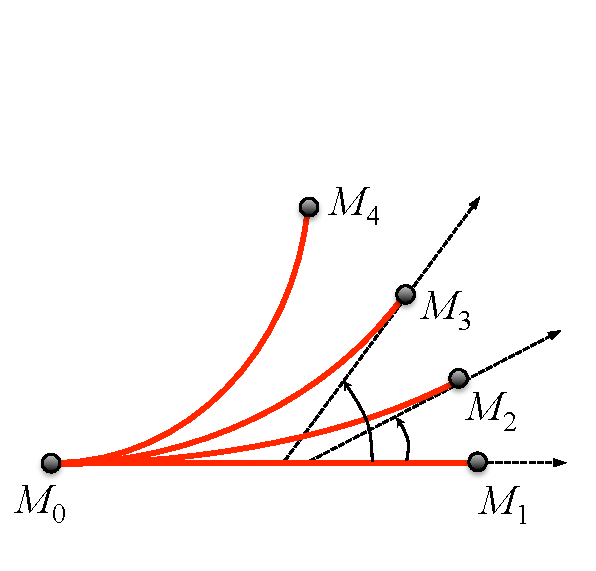
\includegraphics{./images/curves/c103.pdf}}}

				\vspace{-1em}\invisible<1->{{\b 长度相同的曲线,切线

				转角越大弯曲程度越大}}
			\end{center}
		\column{.5\textwidth}
	\end{columns}
\end{frame}

\begin{frame}{曲率}
	\linespread{1.2}
	\centerline{\ba{如何刻画曲线的弯曲程度?}}

	\begin{columns}
		\column{.5\textwidth}
			\begin{center}
				\vspace{-1em}
				{\resizebox{!}{5.5cm}{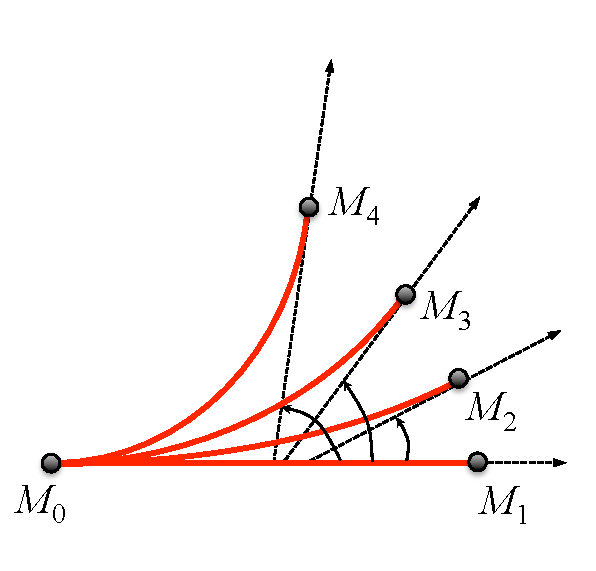
\includegraphics{./images/curves/c102.pdf}}}

				\vspace{-1em}\invisible<1->{{\b 长度相同的曲线,切线

				转角越大弯曲程度越大}}
			\end{center}
		\column{.5\textwidth}
	\end{columns}
\end{frame}

\begin{frame}{曲率}
	\linespread{1.2}
	\centerline{\ba{如何刻画曲线的弯曲程度?}}

	\begin{columns}
		\column{.5\textwidth}
			\begin{center}
				\vspace{-1em}
				{\resizebox{!}{5.5cm}{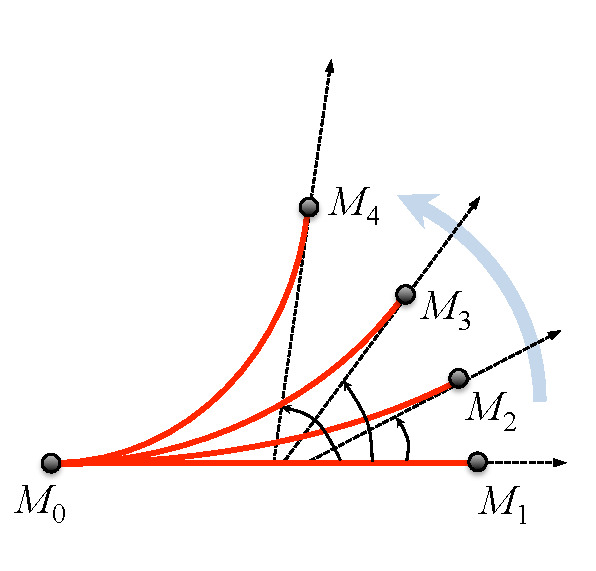
\includegraphics{./images/curves/c101.pdf}}}

				\vspace{-1em}{{\b 长度相同的曲线,切线

				转角越大弯曲程度越大}}
			\end{center}
		\column{.5\textwidth}
	\end{columns}
\end{frame}

% \begin{frame}{曲率}
% 	\linespread{1.2}
% 	\centerline{\ba{如何刻画曲线的弯曲程度?}}
% 
% 	\begin{columns}
% 		\column{.5\textwidth}
% 			\begin{center}
% 				\vspace{-1em}
% 				{\resizebox{!}{5.5cm}{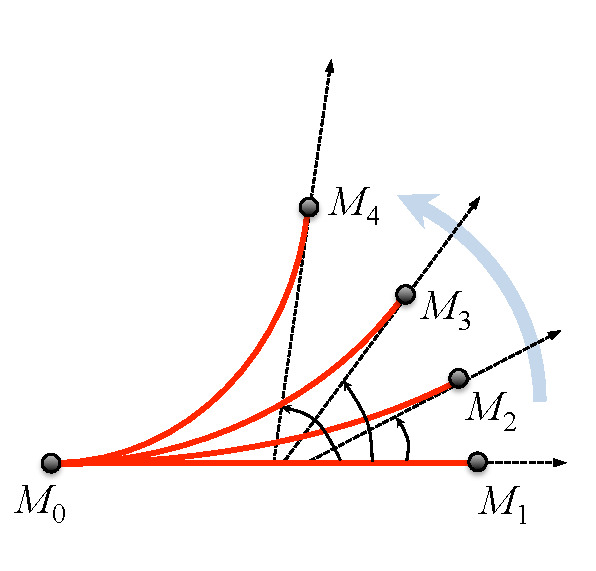
\includegraphics{./images/curves/c101.pdf}}}
% 
% 				\vspace{-1em}{{\b 长度相同的曲线,切线
% 				
% 				转角越大弯曲程度越大}}	
% 			\end{center}
% 		\column{.5\textwidth}
% 			\begin{center}			
% 				\vspace{-1em}
% 				{\resizebox{!}{5.5cm}{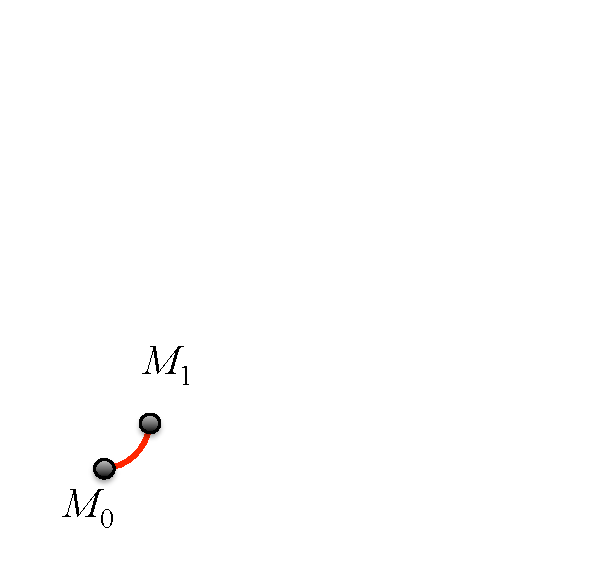
\includegraphics{./images/curves/c208.pdf}}}
% 				
% 				\vspace{-1em}{\color{white} 切线转角相同的曲线,
% 
% 				弧长越短弯曲程度越大}
% 			\end{center}
% 	\end{columns}
% \end{frame}
% 
% \begin{frame}{曲率}
% 	\linespread{1.2}
% 	\centerline{\ba{如何刻画曲线的弯曲程度?}}
% 
% 	\begin{columns}
% 		\column{.5\textwidth}
% 			\begin{center}
% 				\vspace{-1em}
% 				{\resizebox{!}{5.5cm}{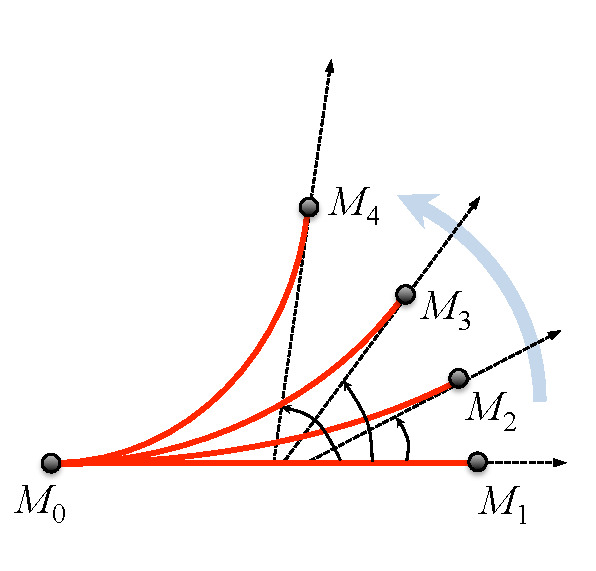
\includegraphics{./images/curves/c101.pdf}}}
% 
% 				\vspace{-1em}{{\b 长度相同的曲线,切线
% 
% 				转角越大弯曲程度越大}}
% 			\end{center}
% 		\column{.5\textwidth}
% 			\begin{center}
% 				\vspace{-1em}
% 				{\resizebox{!}{5.5cm}{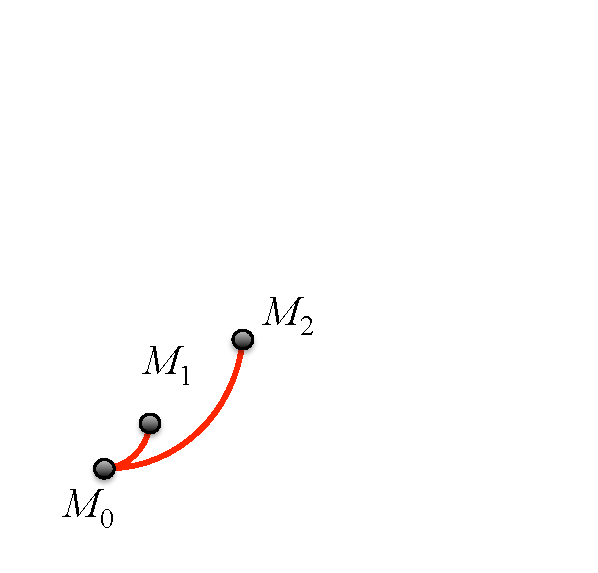
\includegraphics{./images/curves/c207.pdf}}}
% 				
% 				\vspace{-1em}{\color{white} 切线转角相同的曲线,
% 
% 				弧长越短弯曲程度越大}
% 			\end{center}
% 	\end{columns}
% \end{frame}

\begin{frame}{曲率}
	\linespread{1.2}
	\centerline{\ba{如何刻画曲线的弯曲程度?}}

	\begin{columns}
		\column{.5\textwidth}
			\begin{center}
				\vspace{-1em}
				{\resizebox{!}{5.5cm}{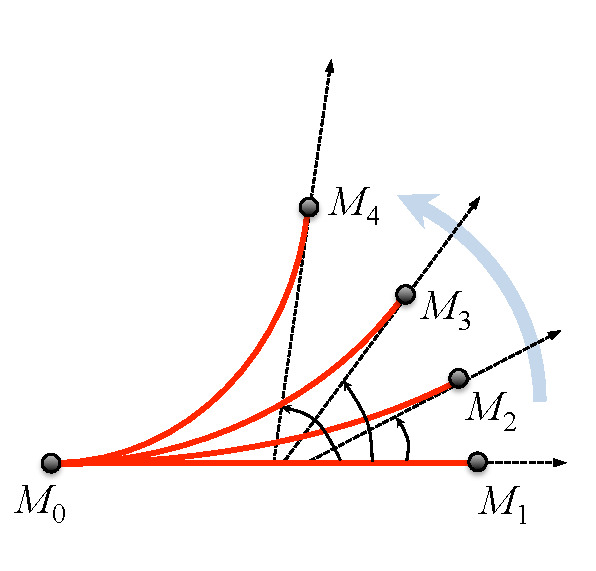
\includegraphics{./images/curves/c101.pdf}}}

				\vspace{-1em}{{\b 长度相同的曲线,切线

				转角越大弯曲程度越大}}
			\end{center}
		\column{.5\textwidth}
			\begin{center}
				\vspace{-1em}
				{\resizebox{!}{5.5cm}{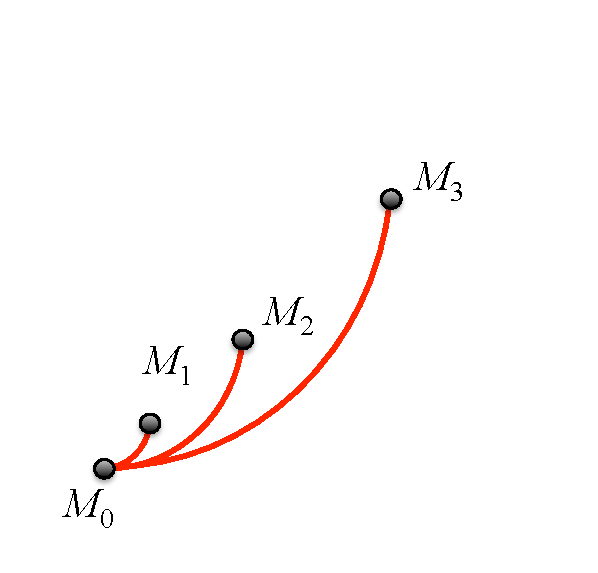
\includegraphics{./images/curves/c206.pdf}}}
				
				\vspace{-1em}{\color{white} 切线转角相同的曲线,

				弧长越短弯曲程度越大}
			\end{center}
	\end{columns}
\end{frame}

\begin{frame}{曲率}
	\linespread{1.2}
	\centerline{\ba{如何刻画曲线的弯曲程度?}}

	\begin{columns}
		\column{.5\textwidth}
			\begin{center}
				\vspace{-1em}
				{\resizebox{!}{5.5cm}{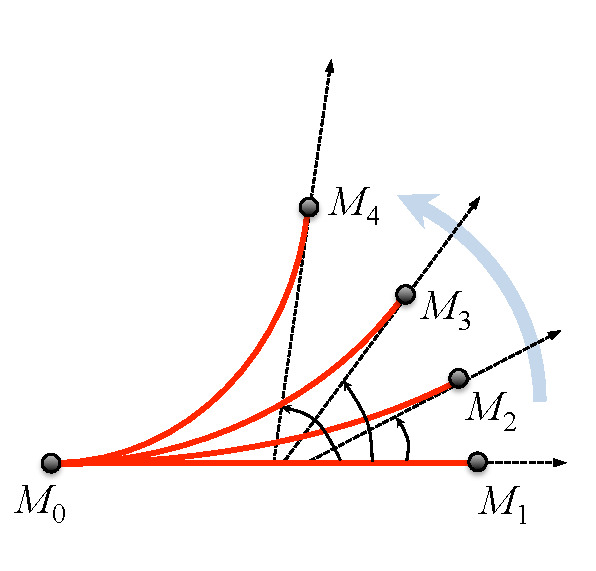
\includegraphics{./images/curves/c101.pdf}}}

				\vspace{-1em}{{\b 长度相同的曲线,切线

				转角越大弯曲程度越大}}
			\end{center}
		\column{.5\textwidth}
			\begin{center}
				\vspace{-1em}
				{\resizebox{!}{5.5cm}{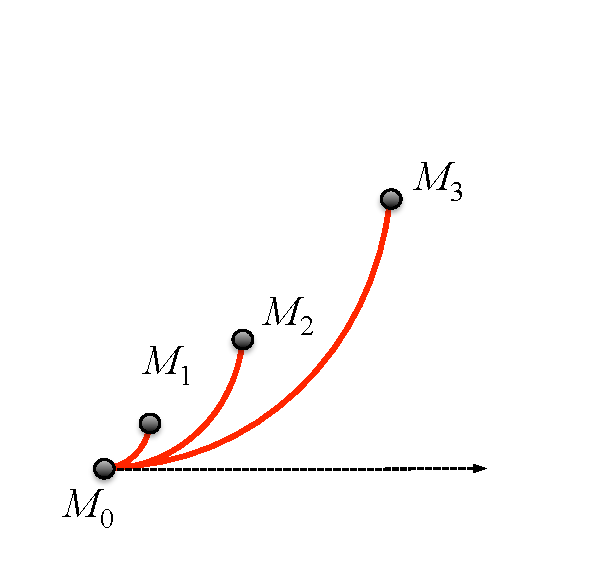
\includegraphics{./images/curves/c205.pdf}}}
				
				\vspace{-1em}{\color{white} 切线转角相同的曲线,

				弧长越短弯曲程度越大}
			\end{center}
	\end{columns}
\end{frame}

\begin{frame}{曲率}
	\linespread{1.2}
	\centerline{\ba{如何刻画曲线的弯曲程度?}}

	\begin{columns}
		\column{.5\textwidth}
			\begin{center}
				\vspace{-1em}
				{\resizebox{!}{5.5cm}{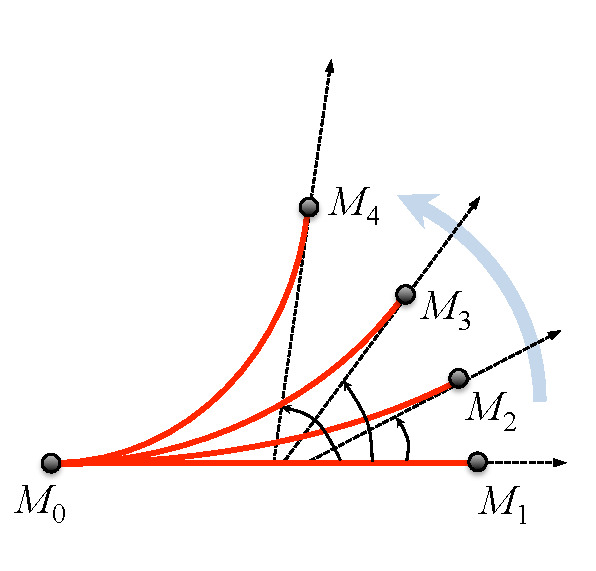
\includegraphics{./images/curves/c101.pdf}}}

				\vspace{-1em}{{\b 长度相同的曲线,切线

				转角越大弯曲程度越大}}
			\end{center}
		\column{.5\textwidth}
			\begin{center}
				\vspace{-1em}
				{\resizebox{!}{5.5cm}{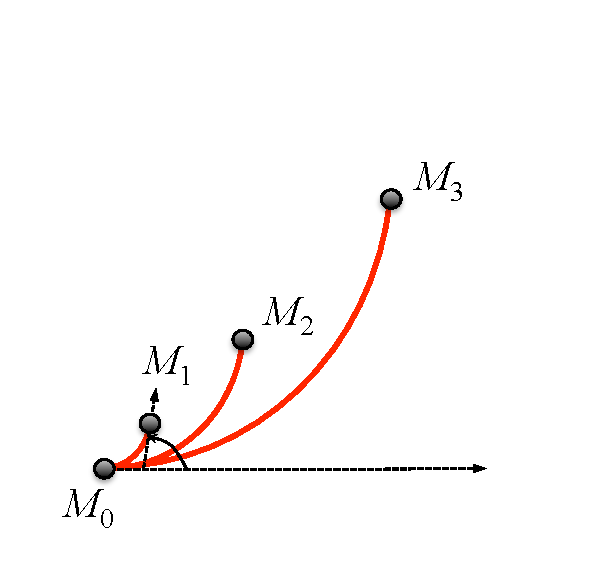
\includegraphics{./images/curves/c204.pdf}}}
				
				\vspace{-1em}{\color{white} 切线转角相同的曲线,

				弧长越短弯曲程度越大}
			\end{center}
	\end{columns}
\end{frame}

\begin{frame}{曲率}
	\linespread{1.2}
	\centerline{\ba{如何刻画曲线的弯曲程度?}}

	\begin{columns}
		\column{.5\textwidth}
			\begin{center}
				\vspace{-1em}
				{\resizebox{!}{5.5cm}{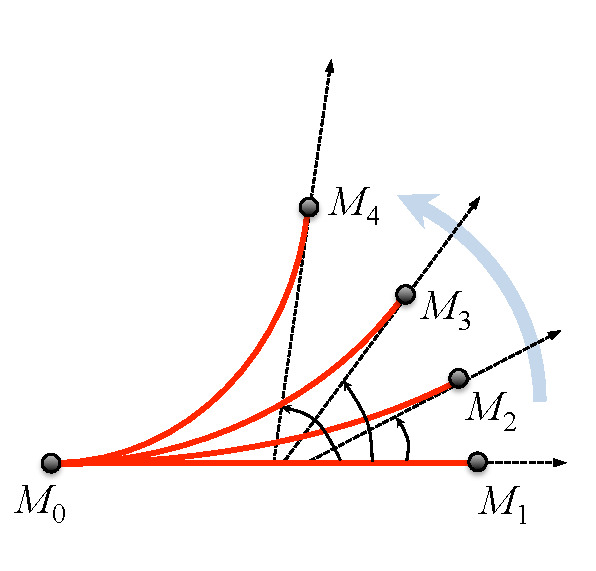
\includegraphics{./images/curves/c101.pdf}}}

				\vspace{-1em}{{\b 长度相同的曲线,切线

				转角越大弯曲程度越大}}
			\end{center}
		\column{.5\textwidth}
			\begin{center}
				\vspace{-1em}
				{\resizebox{!}{5.5cm}{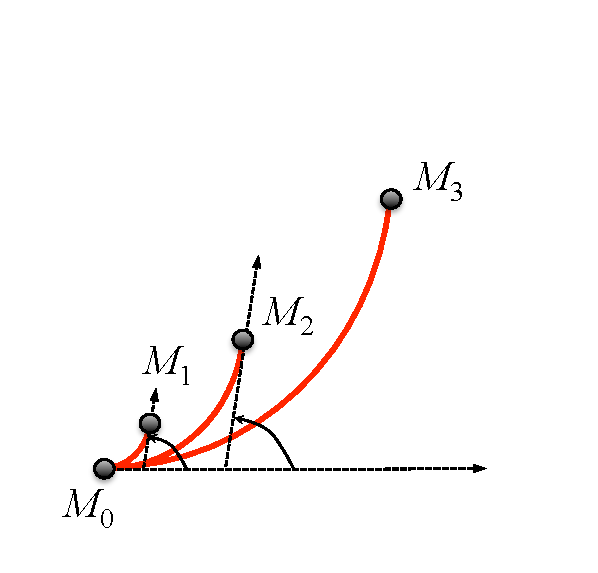
\includegraphics{./images/curves/c203.pdf}}}
				
				\vspace{-1em}{\color{white} 切线转角相同的曲线,

				弧长越短弯曲程度越大}
			\end{center}
	\end{columns}
\end{frame}

\begin{frame}{曲率}
	\linespread{1.2}
	\centerline{\ba{如何刻画曲线的弯曲程度?}}

	\begin{columns}
		\column{.5\textwidth}
			\begin{center}
				\vspace{-1em}
				{\resizebox{!}{5.5cm}{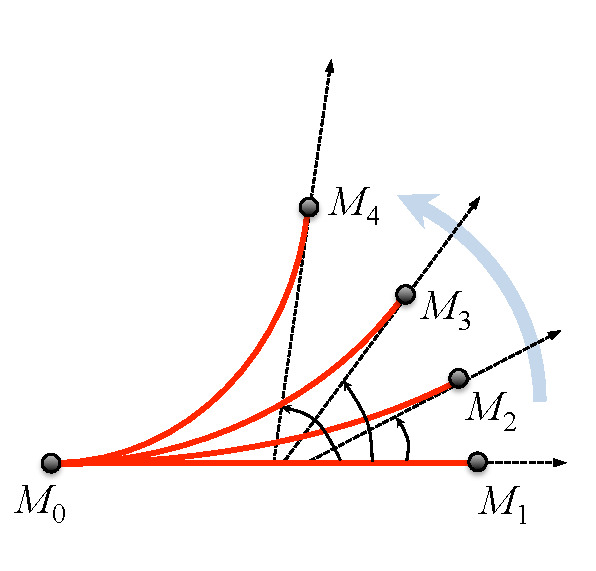
\includegraphics{./images/curves/c101.pdf}}}

				\vspace{-1em}{{\b 长度相同的曲线,切线

				转角越大弯曲程度越大}}
			\end{center}
		\column{.5\textwidth}
			\begin{center}
				\vspace{-1em}
				{\resizebox{!}{5.5cm}{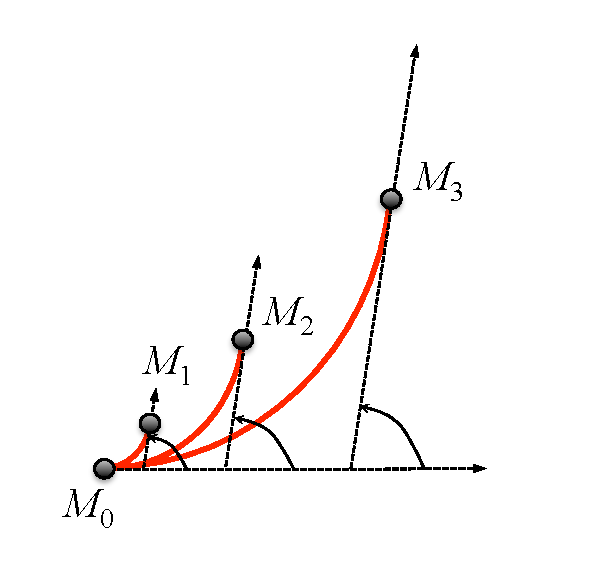
\includegraphics{./images/curves/c202.pdf}}}
				
				\vspace{-1em}{\color{white} 切线转角相同的曲线,

				弧长越短弯曲程度越大}
			\end{center}
	\end{columns}
\end{frame}

\begin{frame}{曲率}
	\linespread{1.2}
	\centerline{\ba{如何刻画曲线的弯曲程度?}}

	\begin{columns}
		\column{.5\textwidth}
			\begin{center}
				\vspace{-1em}
				{\resizebox{!}{5.5cm}{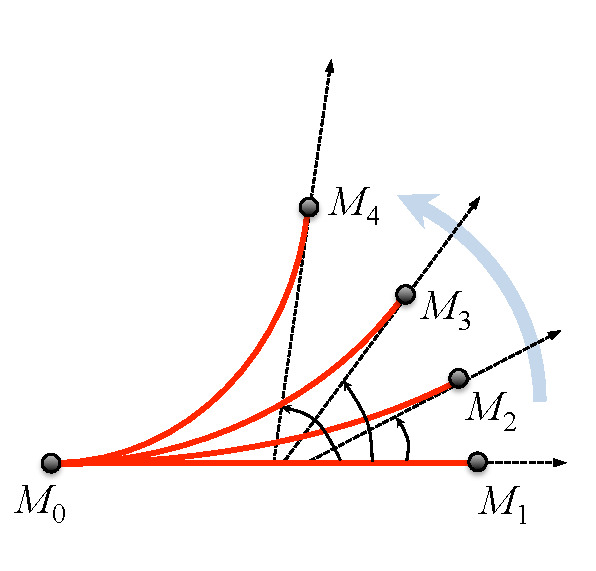
\includegraphics{./images/curves/c101.pdf}}}

				\vspace{-1em}{{\b 长度相同的曲线,切线

				转角越大弯曲程度越大}}
			\end{center}
		\column{.5\textwidth}
			\begin{center}
				\vspace{-1em}
				{\resizebox{!}{5.5cm}{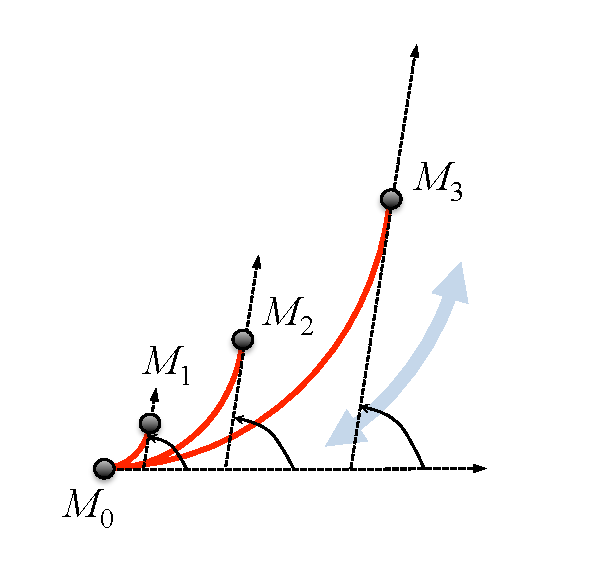
\includegraphics{./images/curves/c201.pdf}}}
				
				\vspace{-1em}{\b 切线转角相同的曲线,

				弧长越短弯曲程度越大}
			\end{center}
	\end{columns}
\end{frame}

%=================================================

\begin{frame}{1、曲率的定义}
	\linespread{1.5}
	\ba{曲线的弯曲程度与切线的转角成正比,弧长成反比}\pause
	\begin{block}{{\bf 定义1}\hfill }
		设曲线$C:y=f(x)$光滑且可求长度,从其上一点$M_0$出发,
		到另一点$M$的弧长
		为$\Delta s$,切线转角为$\Delta\alpha$。
		\pause 若
		
		极限$\lim\limits_{\Delta s\to
		0}\left|\df{\Delta\alpha}{\Delta s}\right|$存在,
		则称之为{\bb 曲线$C$在$M_0$处的曲率},记为
	$$\alert{K=\lim\limits_{\Delta s\to
				0}\left|\df{\Delta\alpha}{\Delta s}\right|\pause
				=\left|\df{\d\alpha}{\d s}\right|}$$ 
	\end{block}
% 	\pause\vspace{-1em}
% 	\begin{itemize}
% 	  \item \alert{曲率:曲线切线的转角关于弧长的变化率}
% 	\end{itemize}
\end{frame}

\subsection{曲率的计算}

\begin{frame}{2、曲率的计算}
	\linespread{1.2}\pause 
	设$y=f(x)$二阶可导,则
	\alert{$$K=\left|\df{d\alpha}{ds}\right|
				\pause =\df{|y''|}{[1+(y')^2]^{3/2}}$$}\pause 
	\begin{exampleblock}{{\bf 例1}\hfill }
		求椭圆$x=3\cos \theta,y=2\sin \theta\,(0\leq \theta\leq 2\pi)$
		上任意点处的曲率,并指出其中曲率最大的点。
	\end{exampleblock} 
\end{frame}

\begin{frame}
	\linespread{1.2}
	\alert{{\bf 注:}根据不同形式的曲线方程,可以得到相应的曲率公式}\pause 
	\begin{enumerate}
	  \item 若曲线由参数方程$\left\{\begin{array}{l}
	  x=x(t)\\ y=y(t)
	  \end{array}\right.$给出,\pause 则
	  $$\alert{K=\df{|x'(t)y''(t)-x''(t)y'(t)|}
		{\{[x'(t)]^2+[y'(t)]^2\}^{3/2}}}$$\pause 
	  \item 若曲线方程为$x=x(y)$,\pause 则
		$$\alert{K=\df{|x''(y)|}{\{[1+[x'(y)]^2\}^{3/2}}}$$
	\end{enumerate}
\end{frame}

\subsection{曲率圆与曲率的应用}

\begin{frame}{3、曲率圆与曲率的应用}
	\linespread{1.2} \pause 
	{\bb 曲率圆:}与已知曲线在凹侧相切,且曲率相同的圆
	
	\pause\vspace{1ex}
	\begin{center}
		\resizebox{!}{4cm}{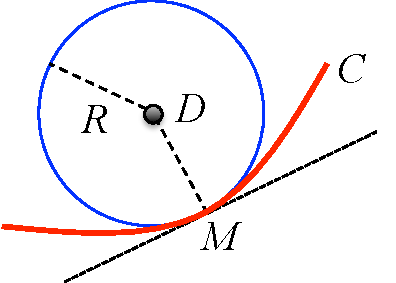
\includegraphics{./images/curSphere.pdf}}
	\end{center}
	\vspace{-1em}\pause 
	\begin{block}{\bf 定理1}
		曲率圆与给定曲线二阶相切。
	\end{block}
\end{frame}

\begin{frame}
	\linespread{1.2} 
	\begin{exampleblock}{{\bf 例2}(加工问题)\hfill }
		已知某工件内侧的截痕曲线为椭圆$\df{x^2}9+\df{y^2}4=1$,
		若用圆形砂轮对其进行打磨,问该如何选择砂轮的尺寸?
	\end{exampleblock}
	\vspace{-1em}
	\begin{columns}
		\column{.55\textwidth}
			\begin{center}
				\only<1>{\resizebox{!}{5.5cm}{
\includegraphics{./images/SE/S0x.pdf}}}%
				\only<2>{\resizebox{!}{5.5cm}{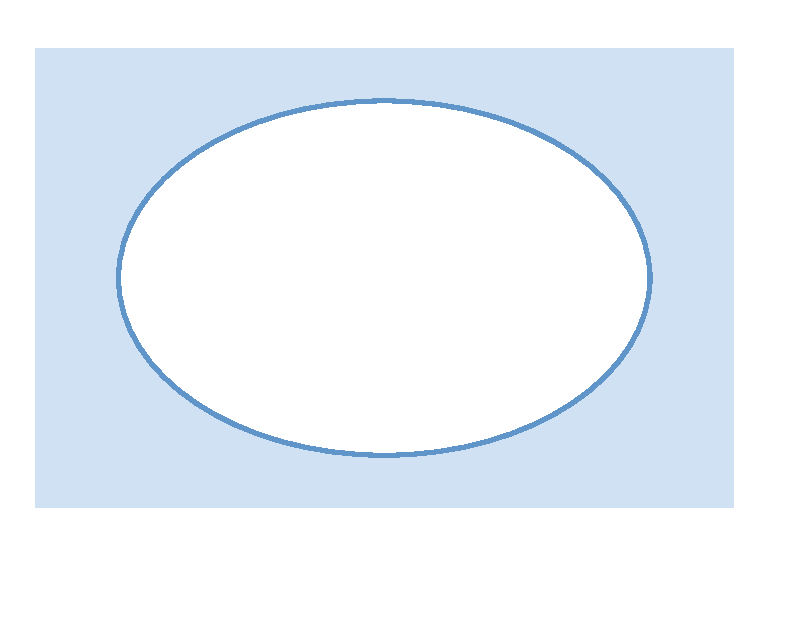
\includegraphics{./images/SE/S05.pdf}}}%
				\only<3-4>{\resizebox{!}{5.5cm}{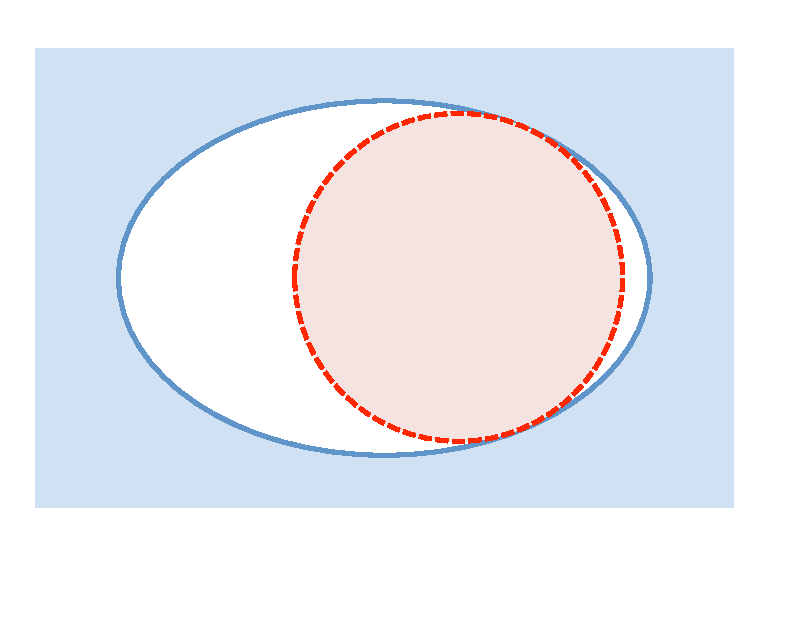
\includegraphics{./images/SE/S04.pdf}}}%
				\only<5-6>{\resizebox{!}{5.5cm}{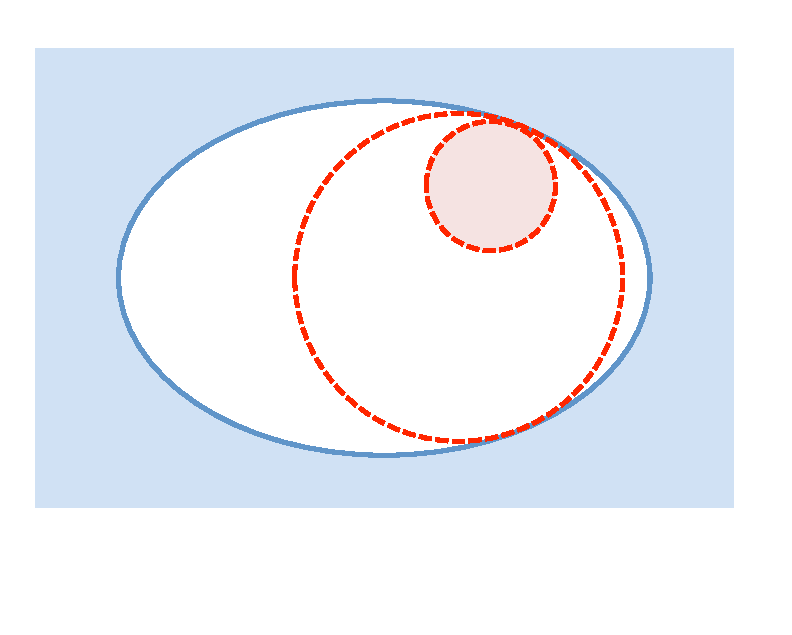
\includegraphics{./images/SE/S03.pdf}}}%
				\only<7-8>{\resizebox{!}{5.5cm}{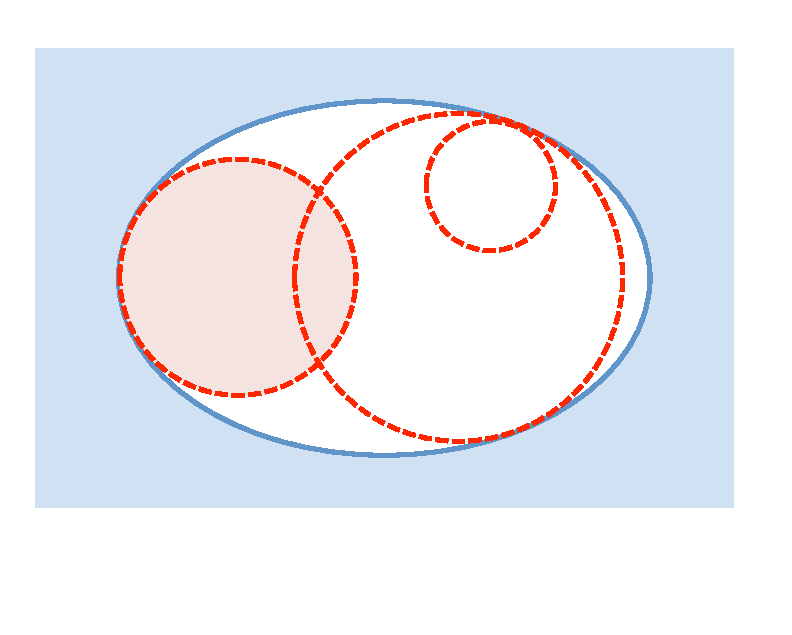
\includegraphics{./images/SE/S02.pdf}}}%
				\only<9>{\resizebox{!}{5.5cm}{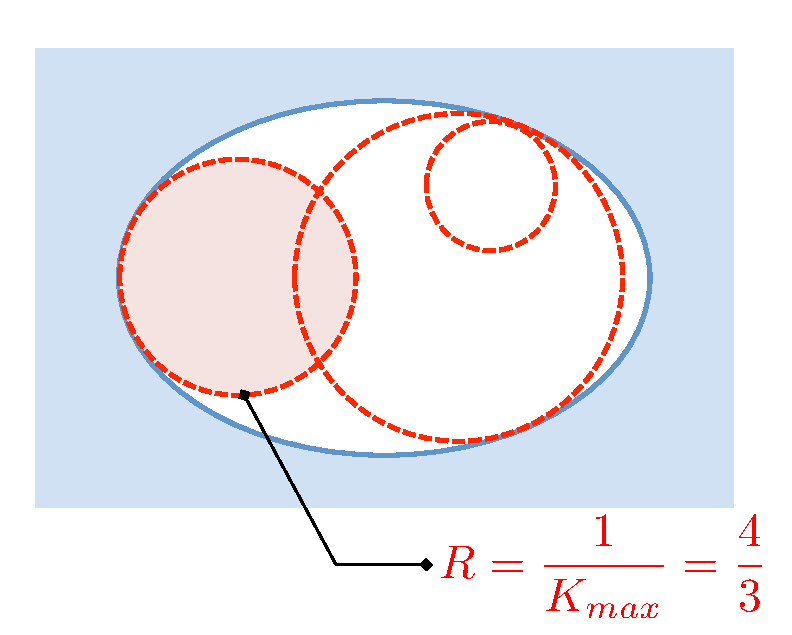
\includegraphics{./images/SE/S01.pdf}}}%
			\end{center}
		\column{.45\textwidth}
			\begin{itemize}
			  \item<4-> 半径过大$\Rightarrow$无法完全打磨
			  \item<6-> 半径过小$\Rightarrow$打磨效率过低
			  \item<8-> {\bf 最优解:}\alert{半径最小的曲率圆}
			\end{itemize}
	\end{columns}
\end{frame}

\begin{frame}{曲率半径与离心力}
	\linespread{1.2}
	\begin{columns}
		\column{.6\textwidth}
			质量为$m$的质点以速度$v$通过光滑曲线上一点,所受离心力为
			$$F=\df{mv^2}{R},$$
			其中$R$为曲线在该点处的曲率半径。
		\column{.4\textwidth}
			\begin{center}
				\resizebox{!}{4.5cm}{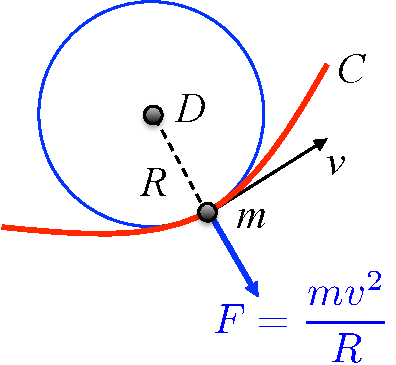
\includegraphics{./images/flip.pdf}}
			\end{center}
	\end{columns}
\end{frame}

\begin{frame}{铁路中的缓和曲线}
	\linespread{1.2}\pause
	\begin{columns}
		\column{.2\textwidth}
			\begin{center}
				\resizebox{!}{1.2cm}{
\includegraphics{./images/train.pdf}}
			\end{center}
		\column{.8\textwidth}
			\ba{为了确保列车行驶安全,尽可能保证列车运行时所受离心力的平稳变化。}\pause 
	\end{columns} 
	\vspace{-1em}
	\begin{columns}
		\column{.65\textwidth}
			\begin{center}
				\only<1-2>{\resizebox{!}{5.5cm}{
\includegraphics{./images/rc00.pdf}}}%
				\only<3-8>{\resizebox{!}{5.5cm}{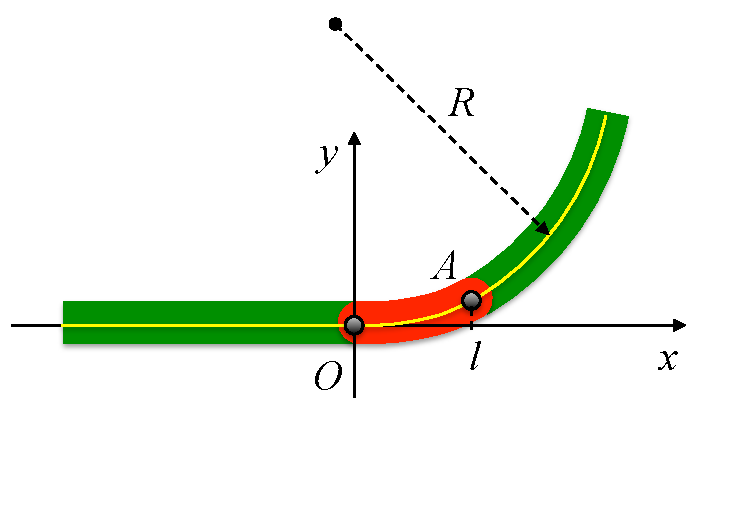
\includegraphics{./images/rc02.pdf}}}%
			\end{center}
		\column{.35\textwidth}
			\uncover<4->{\ba{常用的缓和曲线:}}%
			\begin{itemize}
			  \item<5-> {\b 三次多项式}
			  \item<6-> {\b 渐开螺旋线}
			  \item<7-> {\b 双扭线}
			  \item<8-> {\b \ldots}
			\end{itemize}
	\end{columns}
\end{frame}

\begin{frame}
	\linespread{1.2}
	\begin{exampleblock}{{\bf 例3}(铁路的缓和曲线)}
		如图,列车匀速行进,经过一段直线轨道后,将进入半径为$R$的圆弧轨道。为
		尽量减少列车行驶中所受的离心力冲击,
		试确定一个三次多项式函数实现两段轨道的连接。
	\end{exampleblock}
	\vspace{-1ex}
	\begin{center}
		\only<1>{\resizebox{!}{5.2cm}{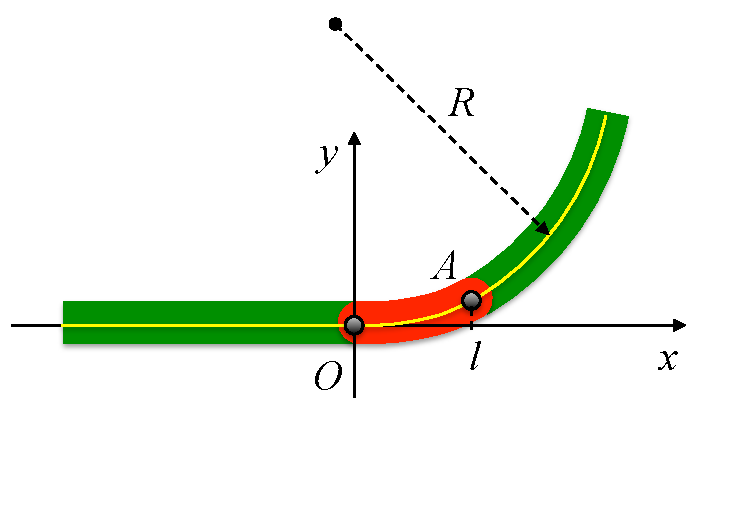
\includegraphics{./images/rc02.pdf}}}%
		\only<2>{\resizebox{!}{5.2cm}{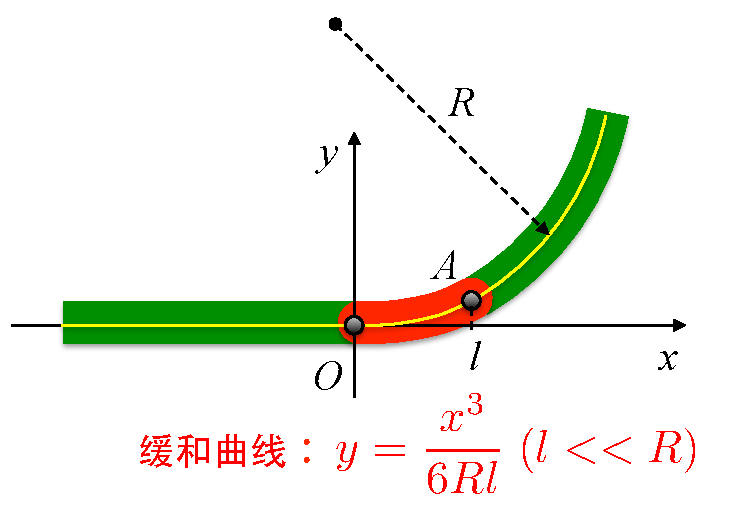
\includegraphics{./images/rc01.pdf}}}%
	\end{center}
\end{frame}

\begin{frame}
	\linespread{1}
	\begin{columns}
		\column{.55\textwidth}
			\resizebox{!}{4.5cm}{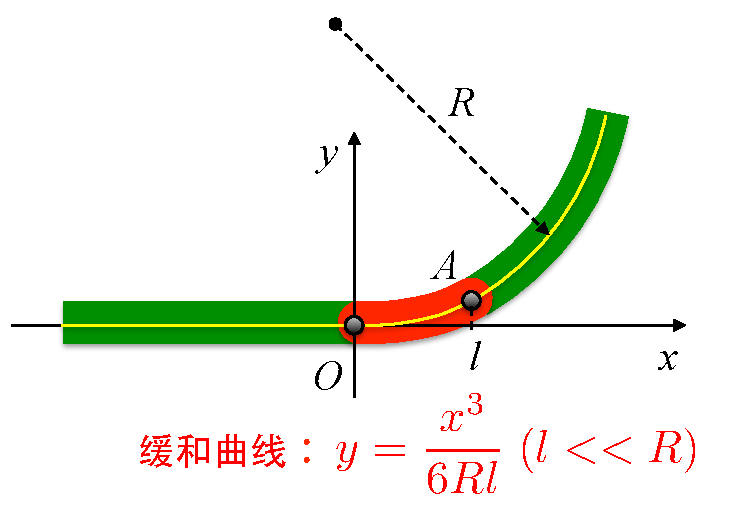
\includegraphics{./images/rc01.pdf}}
		\column{.45\textwidth}
			{\small
			\begin{itemize}
			  \item 匀速行驶$v=108km/h$
			  \item 乘客体重$m=50kg$
			  \item 圆弧半径$R=1000m$
			  \item 缓和曲线长$l=90m$
			\end{itemize}
			}
	\end{columns}
	\vspace{-1em}\pause
	\begin{columns}
		\column{.55\textwidth}
			\begin{center}
				\resizebox{!}{4cm}{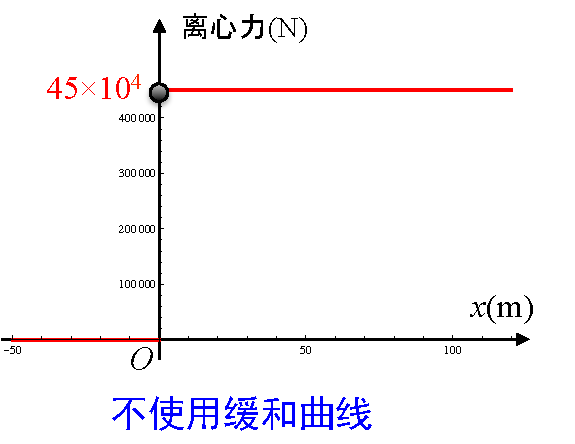
\includegraphics{./images/f01.pdf}}\pause
			\end{center}
		\column{.45\textwidth}
			\begin{center}
				\resizebox{!}{4cm}{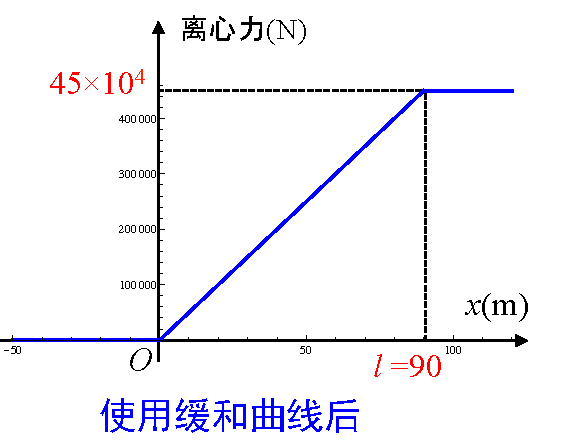
\includegraphics{./images/f02.pdf}}
			\end{center}
	\end{columns}
\end{frame}

\begin{frame}{铁路与轨道交通}
	\linespread{1.2}
	\vspace{-2em}
	\begin{center}
		\hspace{1em}\resizebox{!}{8cm}{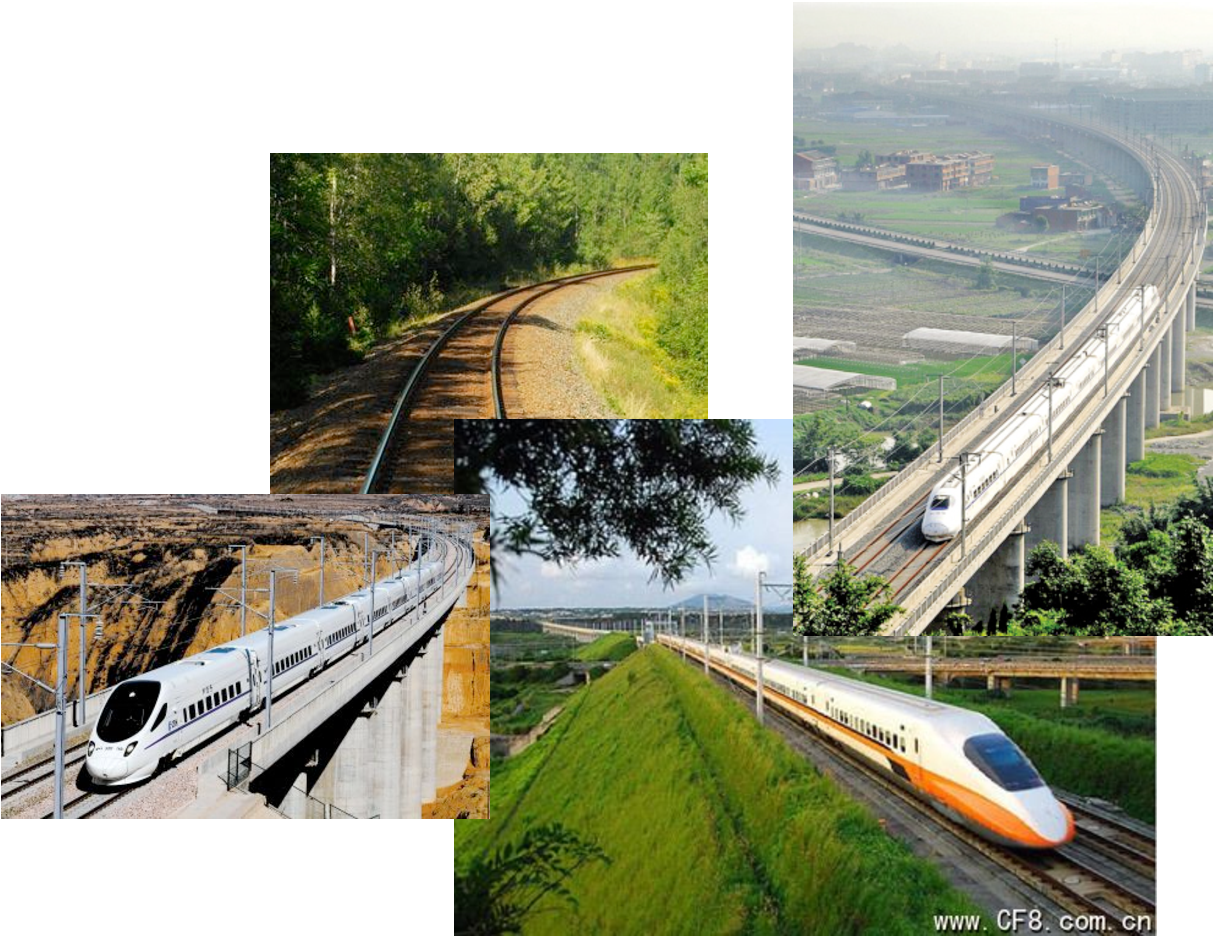
\includegraphics{./images/hr.pdf}}
	\end{center}
\end{frame}

\begin{frame}{高速公路}
	\linespread{1.2}
	\vspace{-1ex}
	\begin{center}
		\hspace{1em}\resizebox{!}{7.2cm}{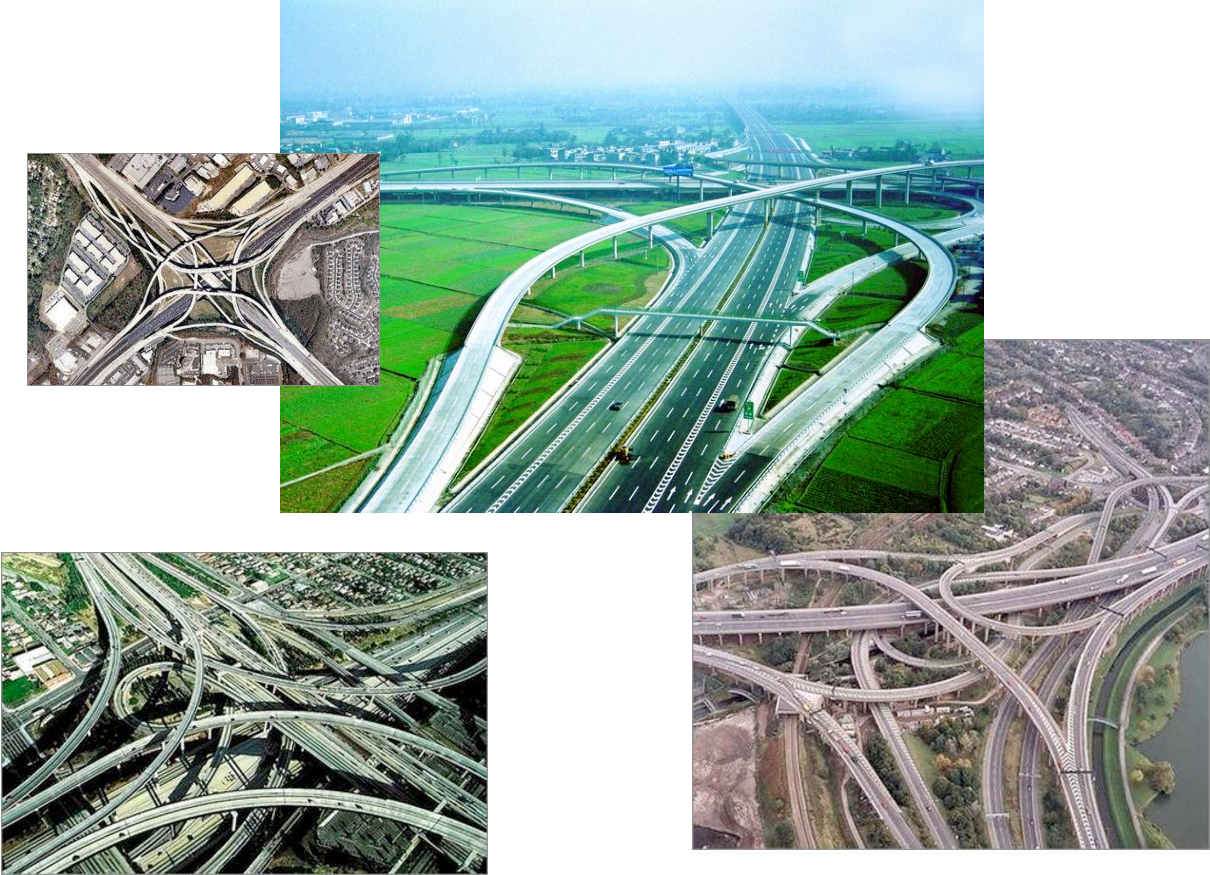
\includegraphics{./images/hw.pdf}}
	\end{center}
\end{frame}

\begin{frame}{过山车}
	\linespread{1.2}
	\vspace{-1ex}
	\begin{center}
		\hspace{1em}\resizebox{!}{7cm}{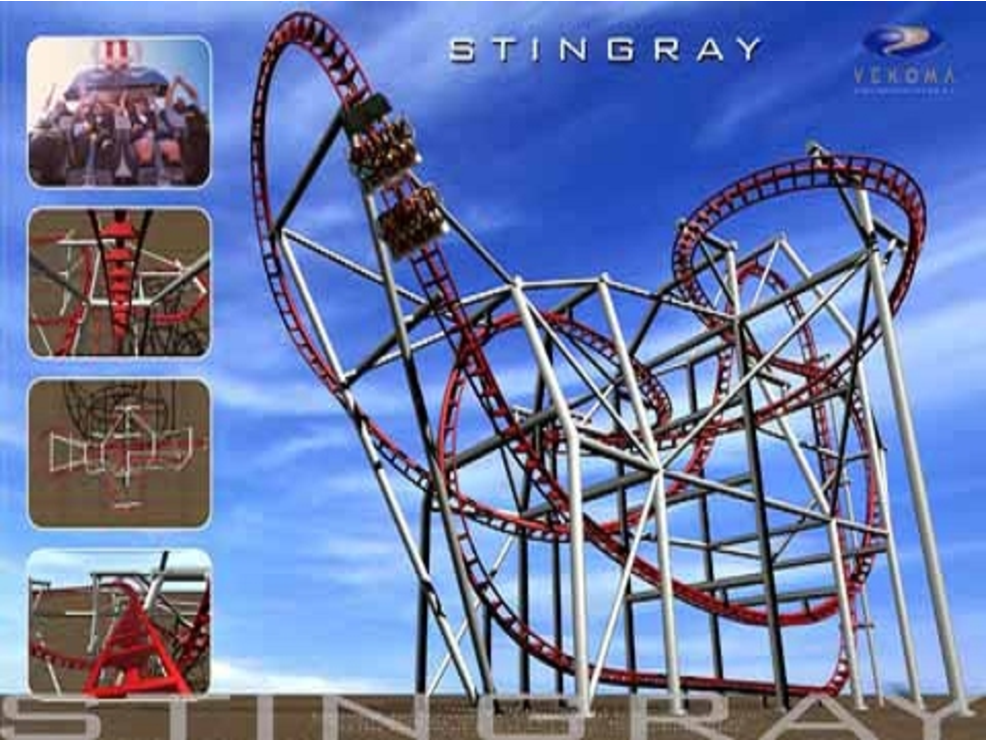
\includegraphics{./images/stg01.pdf}}
	\end{center}
\end{frame}

\begin{frame}{过山车}
	\linespread{1.2}
	\vspace{-1ex}
	\begin{center}
		\hspace{1em}\resizebox{!}{7.2cm}{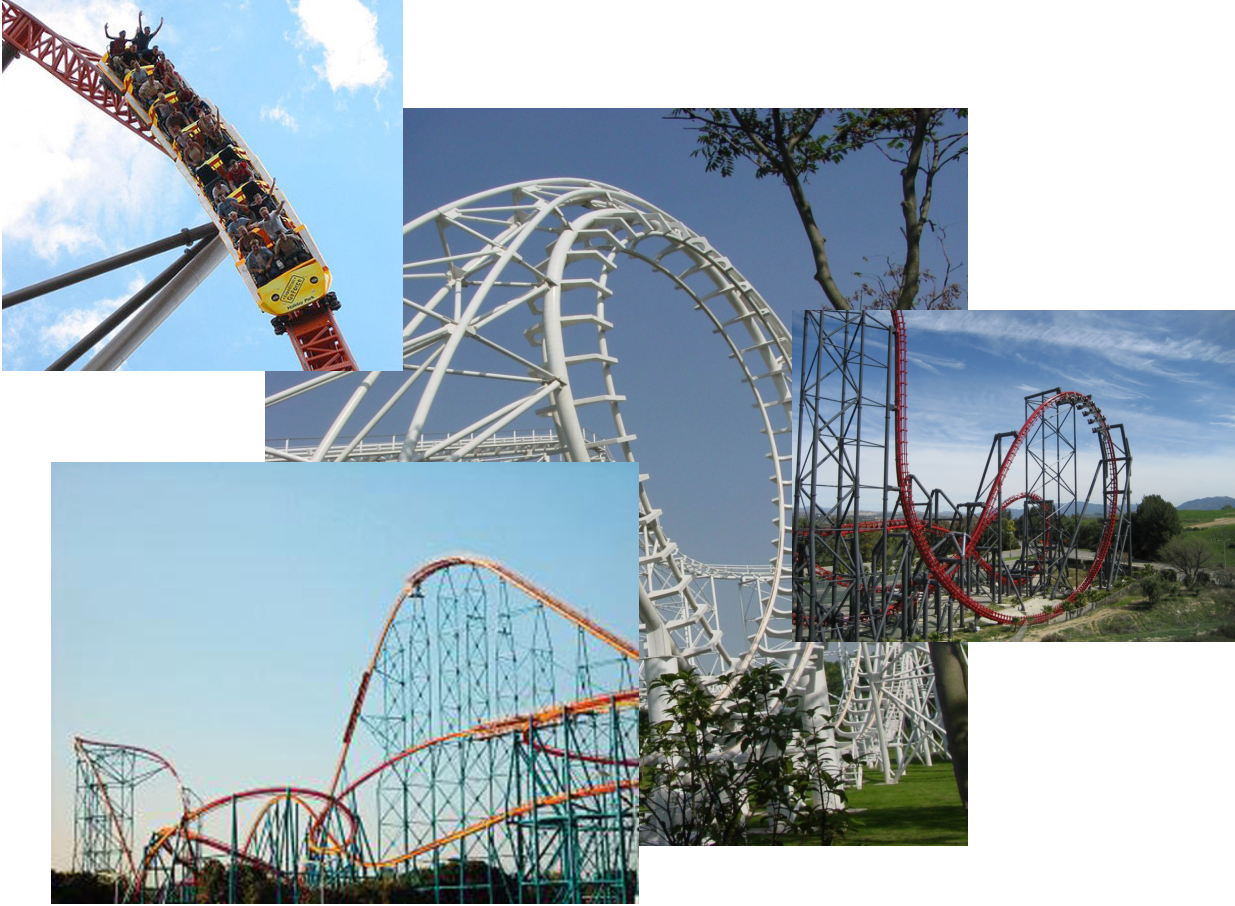
\includegraphics{./images/stg02.pdf}}
	\end{center}
\end{frame}

\begin{frame}{小结}
	\linespread{1.2}
	\begin{enumerate}
	  \item {\bf 曲率的概念:}切线转角相对于弧长的变化率
	  \item {\bf 曲率的计算:}
	  $$\alert{K=\left|\df{d\alpha}{ds}\right|
				=\df{|y''|}{[1+(y')^2]^{3/2}}}$$
	  \item {\bf 曲率圆与曲率的应用}
	  \begin{itemize}
	    \item 曲率半径、离心力与缓和曲线
	  \end{itemize}
	\end{enumerate}
	\pause
	\begin{exampleblock}{{\bf 课后思考题}(过山车设计)\hfill}
		试设计一个分段的多项式函数,完成过山车上一段水平轨道与一段上坡直线轨道的接合。
	\end{exampleblock}
\end{frame}


% \chapter{微分学的应用}

\begin{center}
	{\Huge\bf \;平面曲线的曲率}
	
% 	(授课教员:唐扬斌,理学院数学与系统科学系,2011年4月)
\end{center}
\vspace{2em}
% {\Large\bf 内容与要求:}
% \begin{itemize}
%   \item 理解平面曲线的曲率概念
%   \item 熟练掌握曲率的计算公式
%   \item 理解曲率圆与曲率半径
%   \item 了解曲率的应用
% \end{itemize}
% 
% {\Large\bf 课后作业:}习题5.5:5,6,7,8,11

% \setcounter{section}{-1}
% \section{引入}

{\bf P1\,引入(2min)}
% \marginpar{\bf (引入-3min)}

各位同学,早上好!

今天,我们一起来学习平面曲线的曲率。在这节课中,我们将介绍曲率的定义、曲率的计算方法,
曲率圆以及曲率的一些重要应用。

首先,让我们来看一张图片。这是我们国家正在建设和运行中的高速铁路。

我国是目前世界上在建和投入运营高铁里程数最多的国家。

那么,高速铁路和我们今天要学习的曲率有什么样的关系呢?让我们来看一个简单的例子。

假设我们有一段直线的轨道和一段圆弧型的轨道,假设圆弧轨道的半径为$R$。现在,列车需要从
直线轨道驶入圆弧轨道。为了确保行车的安全,在轨道连接时,我们会让两段轨道在接合处相切。
但是,这样就足够了吗?
\marginpar{\bf (作图分析)}

让我们来分析一下。大家知道,当列车在圆弧轨道上运行时,会受到一个离心力的作用,这个力
的大小与其自身质量、行驶速度以及轨道的半径相关,为$F_{\mbox{离}}=\df{mv^2}{R}$,
方向指向轨道外侧。

另一方面,在直线轨道上运行时,如果假设列车是匀速行驶的,则列车本身应该不会收到任何离心力的作用。

请大家想一想,在列车由直线轨道驶入圆弧轨道的那一刻,列车上的乘客会有什么样的感受?
\marginpar{\bf (提问)}

对!一次冲击!在轨道切换的一刻,乘客会在瞬间受到一个离心力的作用,如果车速很快,这个
冲击将是相当巨大的。由此可见,无论从安全性还是舒适性的角度出发,目前的这种设计都不是
一个好的方案。那么,该如何解决这个问题呢?

通过我们今天的学习,我们将给出这个问题的答案。

\bigskip
{\bf P2\,知识回顾(1min)}

什么是曲线的曲率?不妨让我们回顾一下我们刚刚学习过的内容。

通过对一元函数导数与微分的应用这一章的学习,我们了解到一元函数的导数与微分是我们刻画
平面曲线的几何特征的重要手段。例如:

一阶导数表示的是曲线在某一点处的切线斜率,形象地说,就是曲线在某一点处的倾斜程度;

通过对二阶导数的研究,我们可以了解曲线的凸凹行,它在局部看起来是像“山峰”还是“山谷”;

上一节课我们所学习的弧微分,则给了我们一种求给定曲线长度的手段;

今天,我们所要学习的曲率,将回答曲线几何特征中另一个非常重要的问题,那就是,曲线的弯曲程度。

\bigskip
{\bf P3\,实验观察(5min)}

那么,我们该如何刻画曲线的弯曲呢?或者,换句话说,怎样的曲线可以被称为是更加弯曲的,这种
弯曲的程度该如何定义呢?这里,我们不妨来做一个小小的实验,观察一下在日常生活中我们是如何
定义曲线的弯曲的。

我手里拿的是我们的高数教材。请大家观察它的侧面,目前,我们可以看到它的侧边是一条直线。
现在,我将书页慢慢翻起,这时我们可以看到很多的曲线。我的第一个问题是,在这些曲线中,哪一条
是最弯曲的?

答案应该很明细那,位置越靠上的曲线越弯曲,其中,封面对应的曲线最为弯曲。那么,相对于其他的曲线,
这条最弯曲的曲线有什么样的特征呢?\marginpar{\bf (提问)}

显然,这页纸的右侧端点偏离其原始位置的幅度最大。

下面我们来分析一下,这种偏离该如何从数学上加以刻画。\marginpar{\bf (投影图)}
请大家来看投影上的图形。假设这是我们刚才看到的书页。请大家注意,这是一族长度完全相同的曲线,并且
其左侧的端点也是相同的。不同在于,越弯曲的曲线,右侧端点离直线位置越远。那么,这种远就是指两点
距离吗?

让我们再回到书页上,如果我这样让书页的端点偏离原始的位置,大家看到了什么?

对,一组直线!虽然书页偏离的距离不同,但我们并没有看到预期中的弯曲。这就告诉我们并不是端点的距离
在决定曲线的弯曲程度。

那么,导致这种弯曲差异的原因究竟是什么?我们不妨再仔细观察一下这里的图形,如果我们作出每条曲线右端点
处的切线。不难发现,随着偏离的增加,曲线的切线与直线位置的夹角越来越大,换句话说,越弯曲的曲线,
切线转过的角度越大。如果我们将每条曲线都想象成某个动点的运动轨迹,我想我们不难得出这样的结论:

长度相同的曲线,切线转角越大越弯曲。

让我们再考虑另一种情形,刚才我们保持曲线的长度不变,让其切线转过不同的角度。现在,我们假设有几条外形
相同的曲线,比如说,一组切线转角相同的圆弧。它们的差异在于弧长,相当于同一段圆弧的不同长度的版本。
我的问题是,根据我们日常的经验,哪一条圆弧更弯曲呢?

我们不妨换个角度来思考,为了转过相同的角度,在这些不同的圆弧上,我们分别走了10步、50步和100步,
那么,走那条圆弧时转弯更急呢?显然,是最短的这条。

从这里我们可以看到,如果切线的转角相同,那么曲线越短就越弯曲。

有了这样一些观察,下面我们就给出平面曲线曲率的定义。

\bigskip
{\bf P4\,曲率的定义(4min)}

从刚才的讨论中,我们可以得出这样的结论:曲线的弯曲程度是与切线的转角成正比,弧长成反比的。

那么,我们是如何定义曲率的呢?
\marginpar{\bf (作图)}

假设我们考虑一段这样一段曲线,为了便于讨论,我们假设它是光滑和可求长度的。

对于曲线$C$上取一点$M_0$,假设从$M_0$出发,到另一点$M$的弧长
为$\Delta s$,切线转角为$\Delta\alpha$。于是,我们可以定义曲线$M_0M$上
的平均曲率,也即平均的弯曲程度:

$$\bar{K}=\df{\Delta\alpha}{\Delta s}$$

显然,这个定义反映了我们刚才观察的结论。

但是,我们同时注意到,在同一段曲线上,每个局部的弯曲程度并不一定完全相同。为了更精确地
定义曲线的弯曲,我们该怎么做呢?

假设我们将$M$视为一个动点,让它不断向着$M_0$靠近,这时我们会发现,$M_0M$的平均曲率
所刻画的范围将越来越小,最终,不难想象,当$M$趋于$M_0$时,平均曲率的极限所反映的,
应该恰好是曲线$C$在$M_0$处的弯曲程度。这一思想,类似于我们定义导数时,通过取极限,
使某段曲线上函数值的平均变化率趋于某点处的变化率。

由此,我们得到对曲率的定义:

$$\lim_{\Delta s\to 0}\df{\Delta\alpha}{\Delta s}.$$

特别地,为了对曲线弯曲程度进行比较,我们约定曲率应该是一个正数,也即

$$K=\lim_{\Delta s\to 0}\left|\df{\Delta\alpha}{\Delta s}\right|.$$

这个定义告诉我们,曲率也就是曲线切线的转角关于弧长的变化率。进一步,我们也将曲率表示为

$$K=\left|\df{\d\alpha}{\d s}\right|.$$

下面来验证一下这个定义,我们考虑两类简单的平面曲线:

{(1)\,直线:}直线的切线就是其自身,因此任意两点处切线的倾角相同,转角$\Delta\alpha$始终为$0$,
故$K=0$。这个结论告诉我们:{\bf 直线不弯!}

{(2)\,半径为$R$的圆:}如下图所示,
\begin{center}
	\resizebox{!}{4cm}{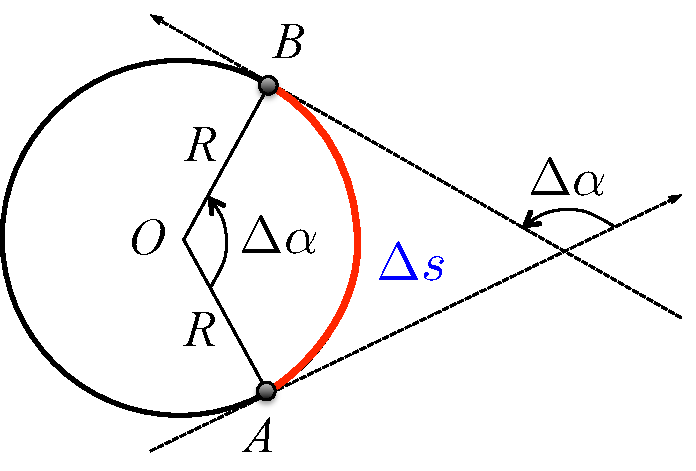
\includegraphics{./images/sphere.pdf}}
\end{center}
$$K=\left|\df{\Delta\alpha}{\Delta s}\right|=\df 1R.$$
这说明,圆的曲率是常数,且唯一依赖于其半径。半径越小的圆,曲率越大。这复合我们此前
通过实验观察得出的结论。
\section{曲率的计算}

下面来看如何计算曲率。假设已知曲线$C$的方程为$y=f(x)$,其中$f(x)$二阶可导,
\marginpar{{\bf 问:}为什么要假设二阶可导?}
则由:
$$\d\alpha=\d\arctan\df yx=\df{y''}{1+(y')^2}\d x,$$
$$\d s=\sqrt{1+(y')^2}\d x,$$
从而
$$K=\df{|y''|}{[1+(y')^2]^{3/2}}.$$
这个定义中,我们注意到分子和分母中分别包含了曲线对应函数的一阶和二阶导数,这说明
曲率和曲线的斜率以及凸凹性直接是存在一定关联的。

下面我们来看一个例题:

{\bf 例1.}\,求椭圆$x=3\cos \theta,y=2\sin \theta\,(0\leq \theta\leq 2\pi)$
上任意点处的曲率,并指出其中曲率最大的点。

{\bf 画图观察:}椭圆上曲率最大的点在什么位置?

{\bf 解:}对任意$\theta\in[0,2\pi]$,
$$y'_x=\df{y'_{\theta}}{x'_{\theta}}=-\df{2\cos\theta}{3\sin\theta}=-\df
23\cot\theta,$$ 
$$y''_{xx}=\df{(y'_x)'_{\theta}}{x'_{\theta}}
=\df23\df{\csc^2\theta}{-3\sin\theta}=-\df 29\csc^3\theta.$$
从而
$$K=\df{|y''_{xx}|}{[1+(y'_x)^2]^{3/2}}=\df 6{(4+5\sin^2\theta)^{3/2}}.$$
显然,当$\theta=0$或$\pi$时,$K$可取到最大值$K_{max}=\df 34$。也即,在椭圆的长轴端点处,
曲率最大。

{\bf 注:}在上面的计算中,我们并没有直接对$y=f(x)$形式的函数求导,而是从曲线的参数方程出发,
利用前面学习过的参数方程求导方法,依次得到了$y'_x,y''_{xx}$和曲率$K$。这种方法,如果给出一个
更为抽象的表示,可以写为:
$$K=\df{|x'(t)y''(t)-x''(t)y'(t)|}
		{\{[x'(t)]^2+[y'(t)]^2\}^{3/2}}.$$

{\bf 课后思考题:}请参照以上的计算方法,推导用$x=x(y)$以及极坐标方程形式表示
的曲线的曲率计算公式。

{\bf 提示:}任何形式的曲线方程都可以被视为曲线参数方程的特殊形式。

\section{曲率圆与曲率的应用}

到目前为止,我们已经定义了曲率的概念,以及计算曲率的公式,下面我们来讨论一下曲率的应用问题。

在此,首先引入所谓{\bf 曲率圆}的概念:\underline{与已知曲线在凹侧相切,且曲率相同的圆}。
\marginpar{{\bf 问:}凹侧该如何理解?}
例如下图:
\begin{center}
	\resizebox{!}{4cm}{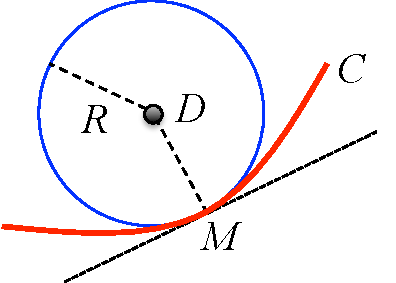
\includegraphics{./images/curSphere.pdf}}
\end{center}
其中蓝色曲线表示的圆与给定曲线$C$在$M$点相切,且二者在$M$点的曲率相同。这样的圆和给定曲线
具有怎样的关系呢?

{\bf 定理1.}\,曲率圆与给定曲线二阶相切。

{\bf 分析:}什么叫“二阶相切”?形象地说,二阶相切是一种比我们熟知的相切“贴合程度”更高的相切。
在介绍切线的概念时,我们曾提到所谓“以直代曲”的概念,也就说在切点附近,由于两者“贴合紧密”,
可以用切线近似地“替代”已知曲线。从上图我们不难看出,曲率圆与已知曲线的“贴合”相对于二者的切线
要更加紧密。

二阶相切在代数上的定义为:若曲线$C_1:y=f(x)$和$C_2:y=g(x)$在$x_0$处同时
满足:
\begin{eqnarray}
	f(x_0)&=&g(x_0),\\
	f'(x_0)&=&g'(x_0),\\
	f''(x_0)&=&''g(x_0).
\end{eqnarray}
假设以上的$C_1$和$C_2$分别为已知曲线和曲率圆。由于二者相切,显然公式$(1)(2)$都是满足的。又
二者的曲率
$$K_1=\df{|f''(x_0)|}{\{1+[f'(x_0)]^2\}^{3/2}}=\df{|g''(x_0)|}{\{1+[g'(x_0)]^2\}^{3/2}}=K_2,$$
故必有$|f''(x_0)|=|g''(x_0)|$。再由二者的“凹侧相切”可知,它们的凹向相同,也即二阶导数同号,
因此$(3)$也满足。

由以上的推导,我们可以很容易地得到一个结论,即曲率圆的半径,也称为已知曲线的{\bf 曲率半径}
$$R=\df 1K.$$
显然,圆的曲率半径就是其半径。

{\bf 应用一:加工问题}
请大家观察我们上面给出的图形,曲线$C$和它对应的曲率圆的位置关系是否很像砂轮和工件表面的曲线呢?
一起来看下面的例子:
{\bf 例2.}\,已知某工件内侧的截痕曲线为椭圆$\df{x^2}9+\df{y^2}4=1$,
若用圆形砂轮对其进行打磨,问该如何选择砂轮的尺寸?
\begin{center}
	\resizebox{!}{4cm}{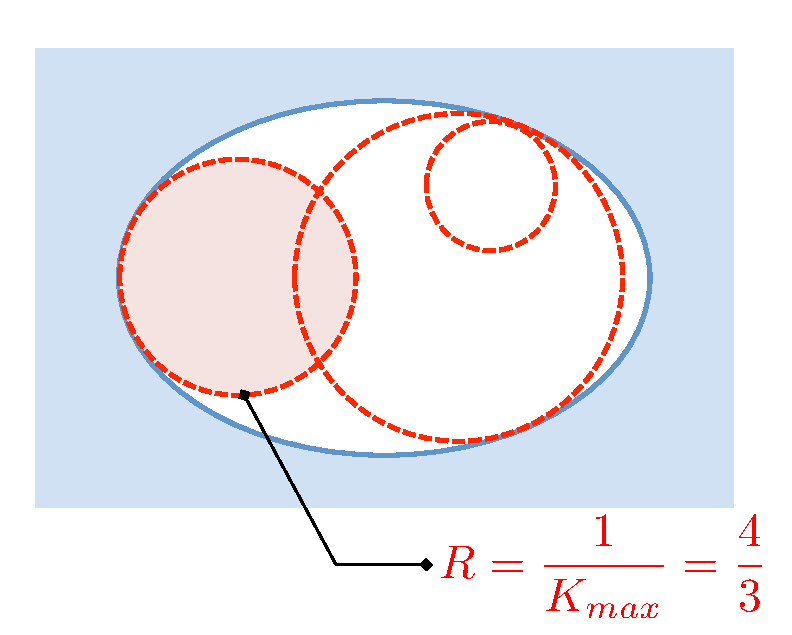
\includegraphics{./images/SE/S01.pdf}}
\end{center}
{\bf 分析:}
\begin{itemize}
  \item 如果选择的砂轮半径过大,工件内部将无法完全被打磨到;
  \item 如果过小,打磨的效率可能相对较低;
  \item {\bf 最优解:}选择曲率半径最小的曲率圆。
\end{itemize}

下面,让我们回到本节课开始时提到的应用问题:

{\bf 应用二:铁路的缓和曲线}

在铁路的设计中,一个重要的原则是:{\bf 为了确保列车行驶安全,应尽可能保证列车运行时
所受离心力的平稳变化。}其中,对于给定曲线上,离心力的计算公式为
$$F=\df{mv^2}{R},$$
其中的$R$为曲线上该点处的曲率半径。

为了解决我们前面提到的问题,在实际的铁路和轨道交通设计中,采用了所谓设置{\bf 缓和曲线}
的方法。也即,在两段曲率不同的轨道间,铺设一段特定的轨道,实现曲率,最终也就是离心力,
的平稳变化。原理如下图所示:
\begin{center}
	\resizebox{!}{5.5cm}{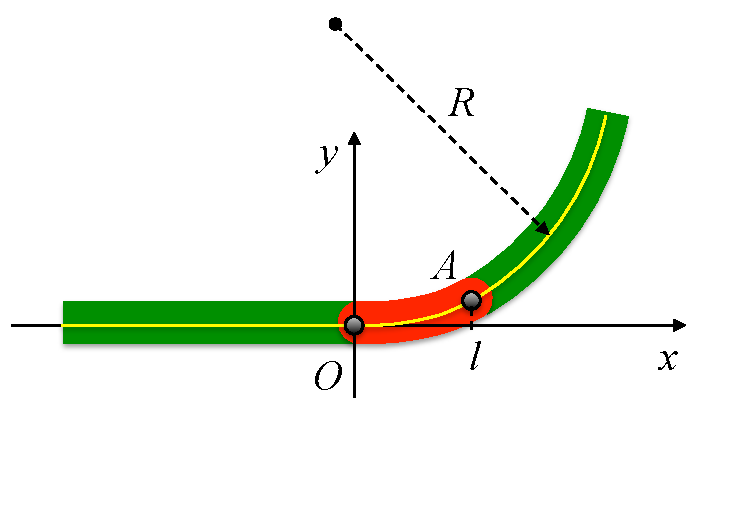
\includegraphics{./images/rc02.pdf}}
\end{center}
图中红色的部分就是我们所说的“缓和曲线”。在工程实践,缓和曲线的设计方式非常多种多样,
其中,较为常见的缓和曲线类型为:
\begin{itemize}
  \item 三次多项式
  \item 渐开螺旋线
  \item 双扭线
\end{itemize}
等等。以下,我们就是三次多项式为例,来考虑如何求解处所需的缓和曲线方程:

{\bf 例3.}\,如上图所示,列车匀速行进,经过一段直线轨道后,将进入半径为$R$的圆弧轨道。为
尽量减少列车行驶中所受的离心力冲击,试确定一个三次多项式函数实现两段轨道的连接。

{\bf 解:}如图建立平面直角坐标系。假设缓和曲线的方程为:
$$y=ax^3+bx^2+cx+d,\quad(a>0,0\leq x\leq l).\eqno{(4)}$$
根据设计原则,在$O$点处,
\begin{eqnarray*}
	y(0)&=&d=0,\\
	y'(0)&=&c=0,\\
	y''(0)&=&b=0.
\end{eqnarray*}
由此,方程$(4)$可简化为$y=ax^3$。

再来考虑点$A$处。注意到为了保证轨道的平滑结合,对于圆弧轨道需要进行一定的“裁剪”和
“平移”,从而保证圆弧曲线和接合曲线在接合点处相切。因此,为了求得参数$a$,我们只需
考虑最后一个约束条件,即:两天曲线在接合点处的二阶导数相同,也即:
$$y''(l)=\df{6al}{(1+9a^2l^4)^{3/2}}=\df 1R.$$
在工程实际中,铁路上的圆弧轨道半径通常为km量级,而缓和曲线的长度会远远小于该值,因此
对上式我们可以做一个近似的求解,得到:$a\approx \df 1{6Rl}$,从而所求缓和曲线为:
$$y=\df{x^3}{6Rl},\quad(0\leq x\leq l).$$

{\bf 计算检验:}为了更好地指导工程设计,在缓和曲线的设计上,已经形成了一整套相关
的规范和标准,例如我国2003年颁布的《地铁设计规范》(GB50157-2003)。我们从其中
取出一组数字,来验证一下我们以上设计的合理性:

假设:列车匀速行驶,车速为$108km/h$,乘客体重$50kg$,圆弧半径$1km$,缓和曲线
长度$90m$,以下是采用缓和曲线前后乘客所受离心力随距离的变化情况:
\begin{center}
	\resizebox{!}{5cm}{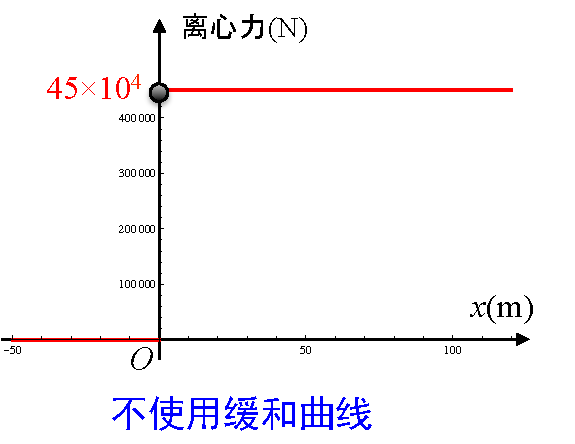
\includegraphics{./images/f01.pdf}}\quad
	\resizebox{!}{5cm}{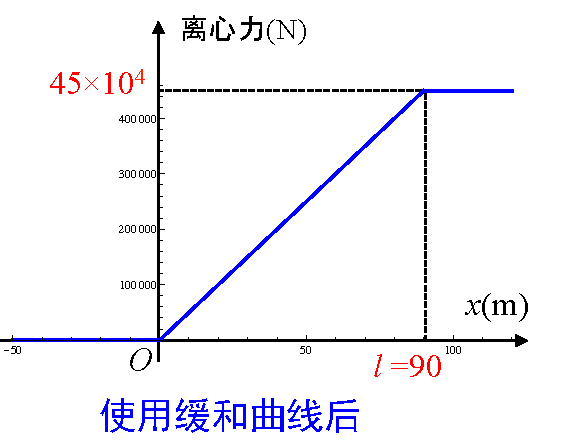
\includegraphics{./images/f02.pdf}}
\end{center}
其中,在不是用缓和曲线的情况下,$45N$(约$5kg$)的离心力将瞬间作用于乘客的身体。
\marginpar{{\bf 提示:}相当于10本高数教材!}
而使用了缓和曲线后,离心力将在3秒内渐次提高,大大降低了乘客所承受的冲量。

{\bf 应用推广:}铁路中的缓和曲线设计,如果概括成一般的数学问题,应该被称为
{\bf 曲线的接合问题}。类似这样的问题,在工程实践中广泛地存在,除了我们这里提到的
铁路与轨道交通,在高速公路设计,甚至是过山车的设计中也存在类似的问题。

{\bf 课后思考题:}(过山车设计)试设计一个分段的多项式函数,完成过山车上一段水平轨道与一段上坡直线轨道的接合。
\end{document}

